\chapter{\label{sec:additionalresults}Additional Results}

\begin{figure}[h]
\centering
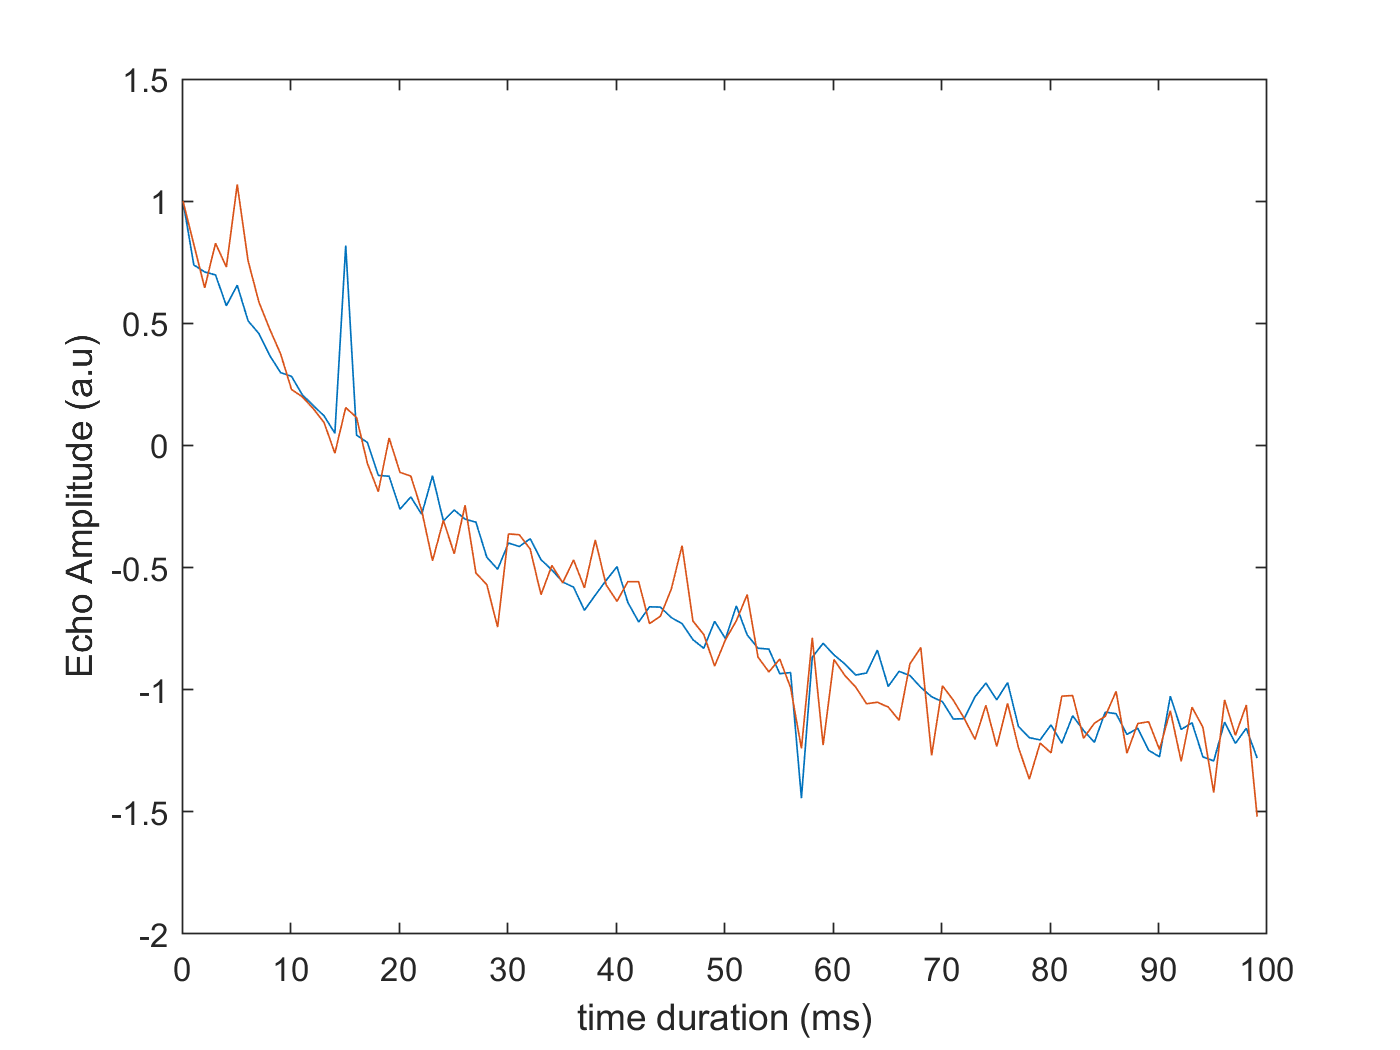
\includegraphics[height=0.5\textwidth,keepaspectratio]{T1naturalSi}
\caption{\label{fig:T1naturalSi} Inversion recovery pulse sequence of natural Si doped with P to determine $T_{1} \approx 20$ ms. The in-phase (I) and out-of-phase (Q) signals are shown in blue and red, respectively.}
\end{figure}

\begin{figure}[H]
    \centering
    \begin{subfigure}[b]{0.45\textwidth}
        \centering
        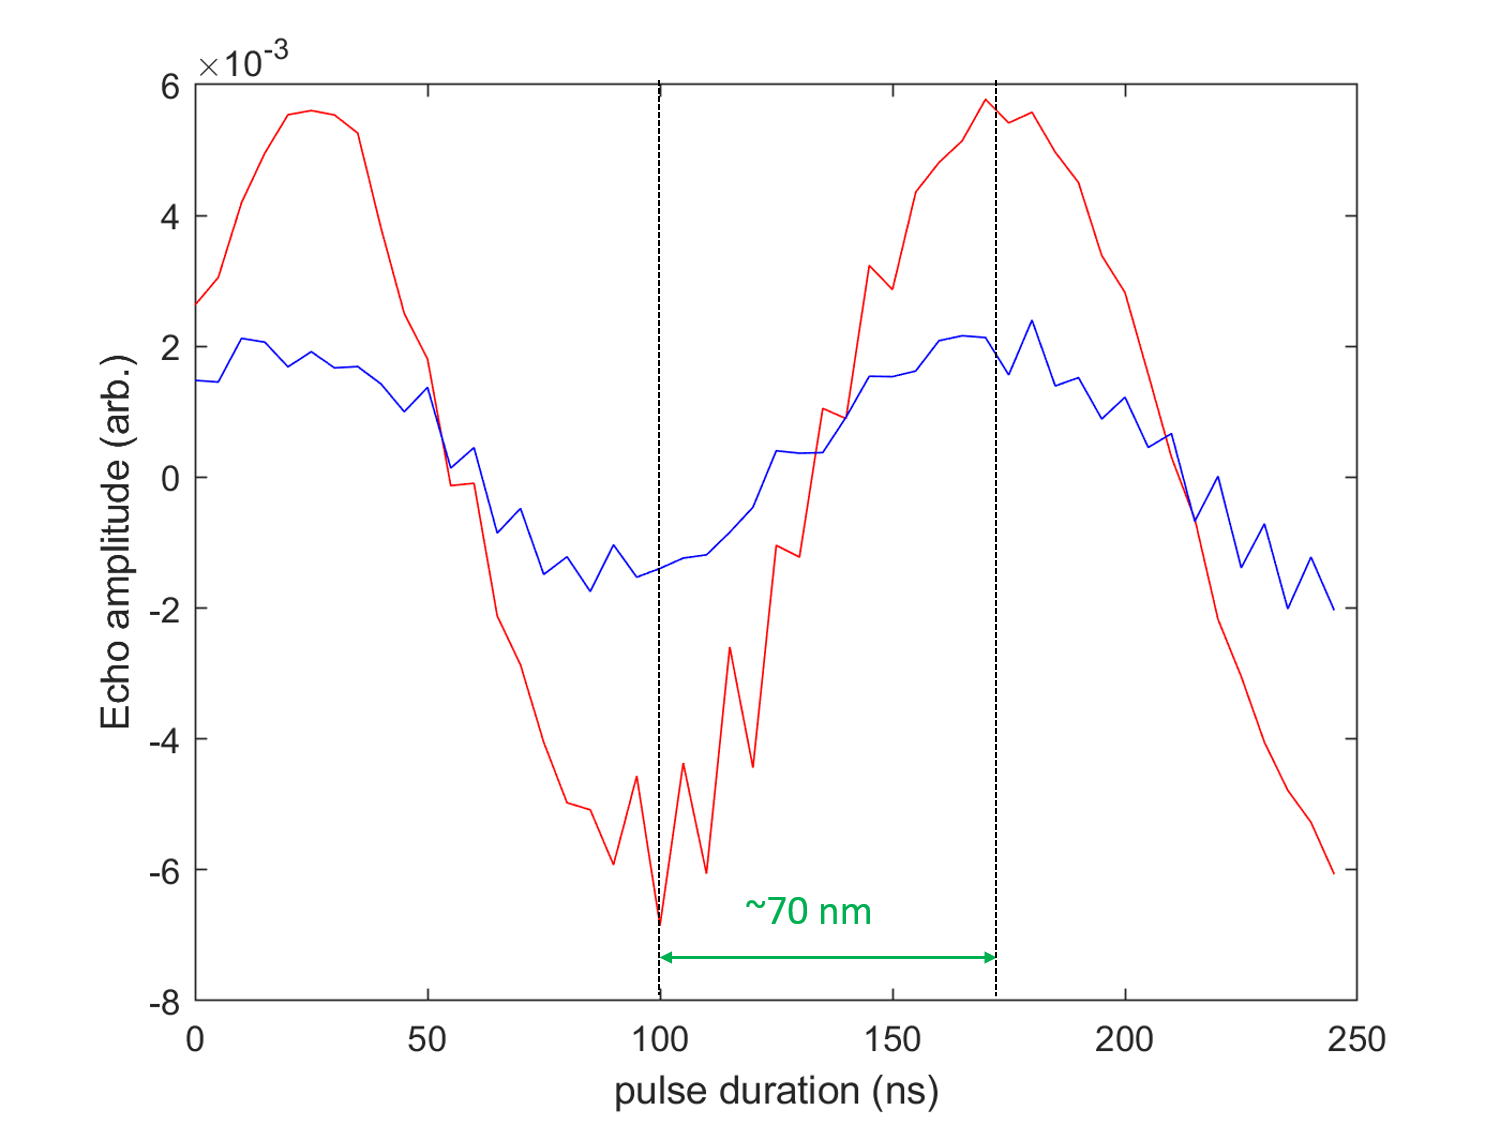
\includegraphics[width=\textwidth]{YbYSORabi}
        \caption{\label{fig:YbYSORabi}}
    \end{subfigure}
%     \hfill
    \begin{subfigure}[b]{0.45\textwidth}
        \centering
        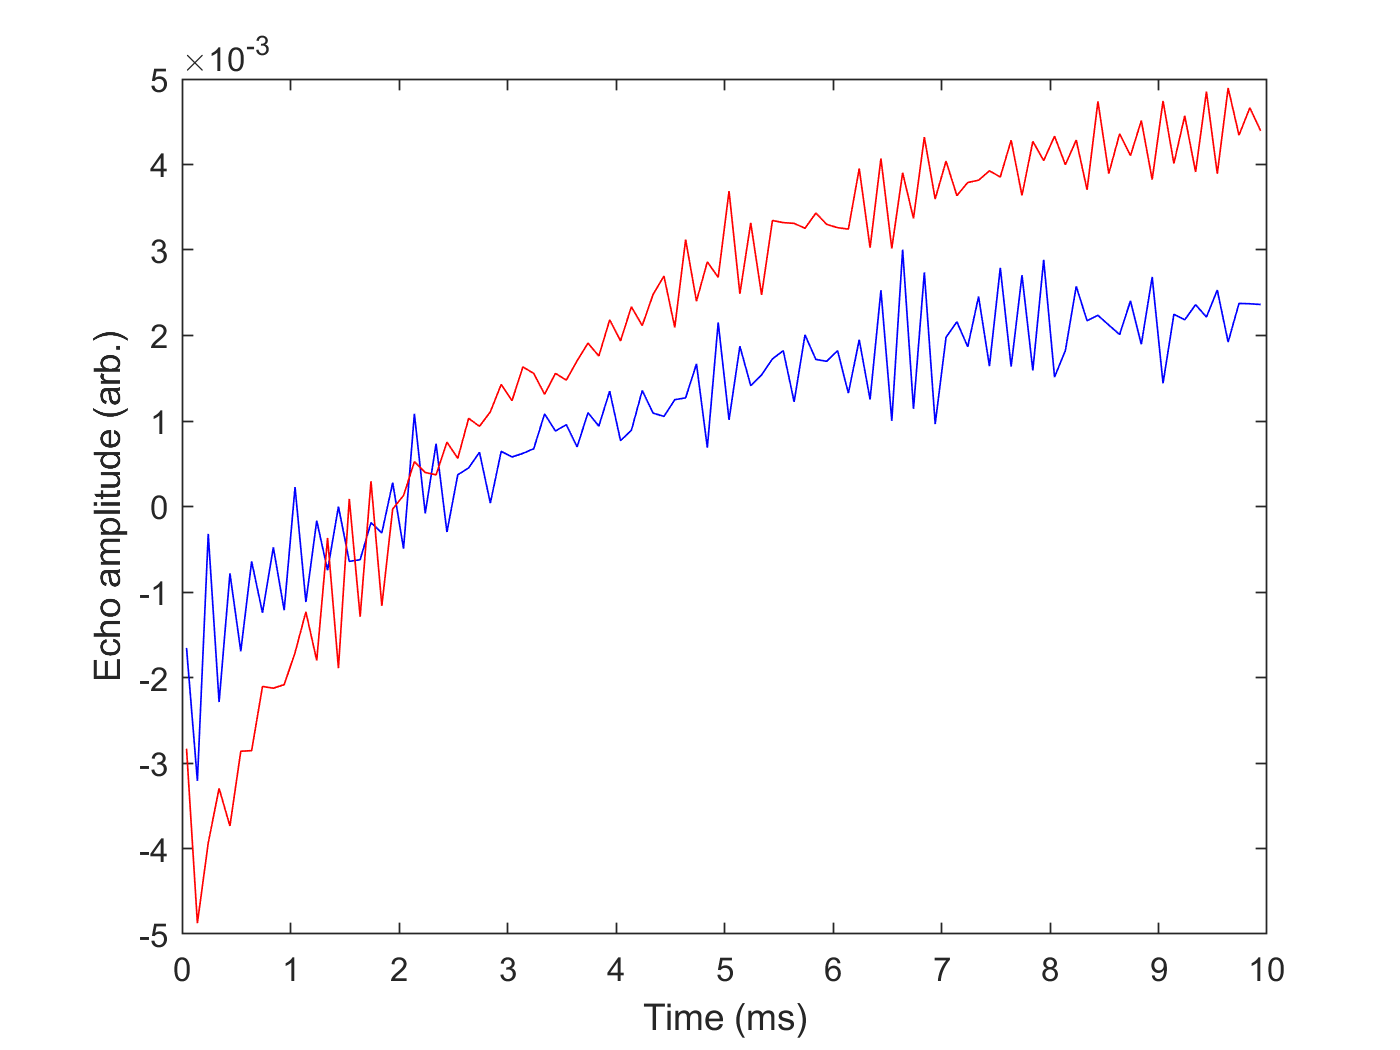
\includegraphics[width=\textwidth]{YbYSOT1}
   \caption{\label{fig:YbYSOT1}}
   \end{subfigure}
   \begin{subfigure}[b]{0.45\textwidth}
        \centering
        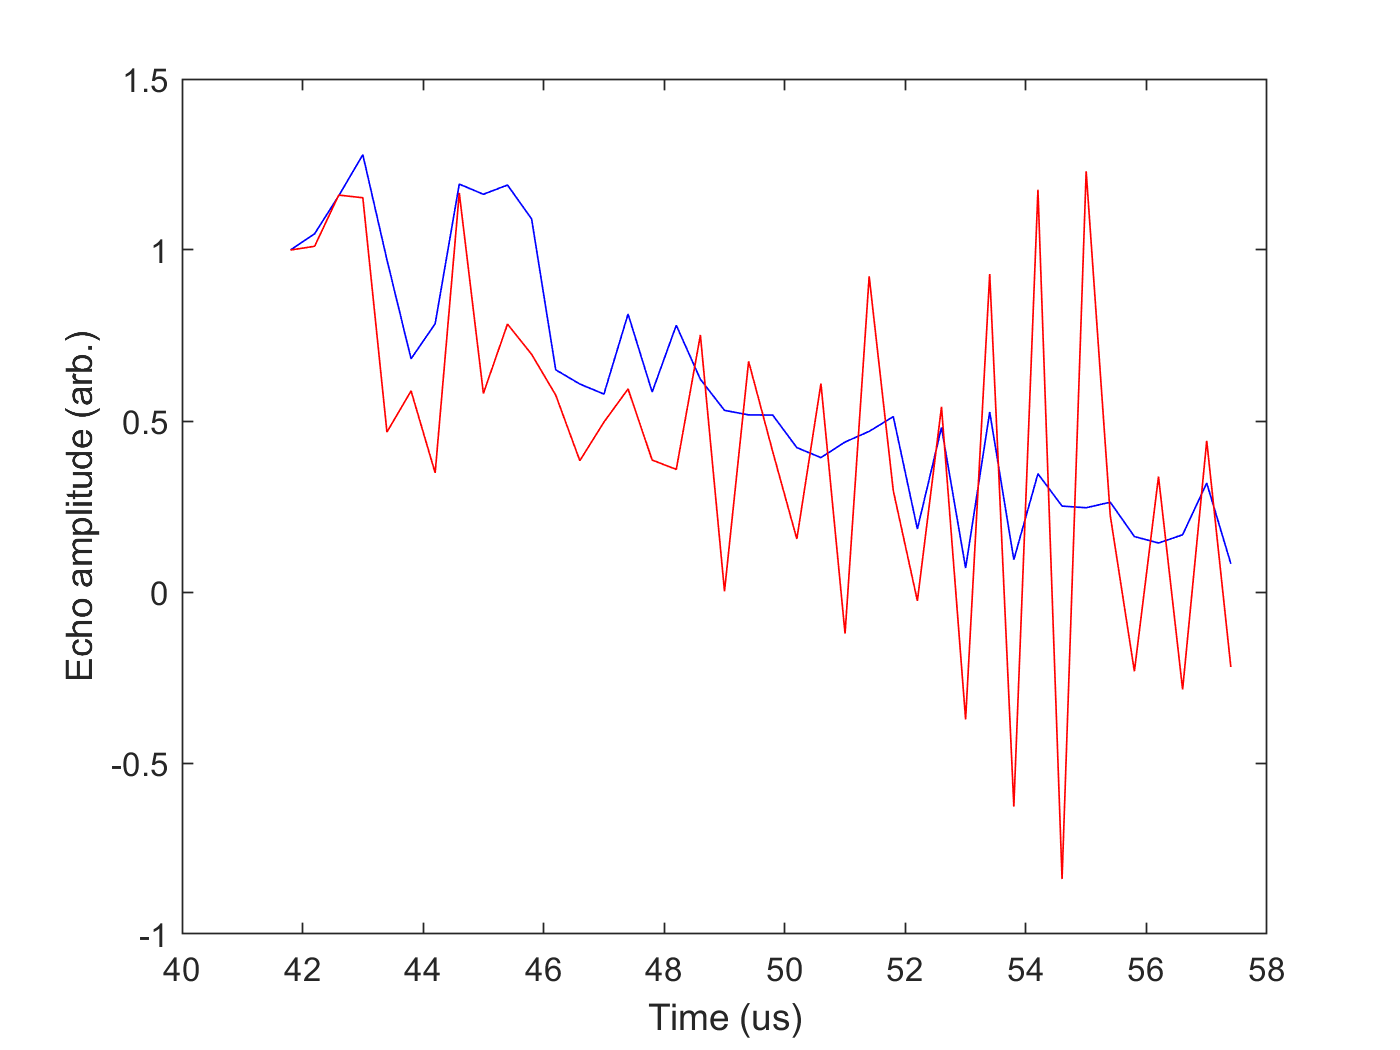
\includegraphics[width=\textwidth]{YbYSOT2}
        \caption{\label{fig:YbYSOT2}}
    \end{subfigure}
    \caption{$^{171}$Yb$^{3+}$:YSO site II (a) Rabi oscillations, (b) $T_{1}$ relaxation curve where $T_{1}\approx 2.6$ ms and (c) $T_{2}$ relaxation curve where $T_{2} \approx 9$ $\mu$s. The in-phase (I) and out-of-phase (Q) signals are shown in blue and red, respectively.}
\end{figure}


\begin{figure}[h]
\centering
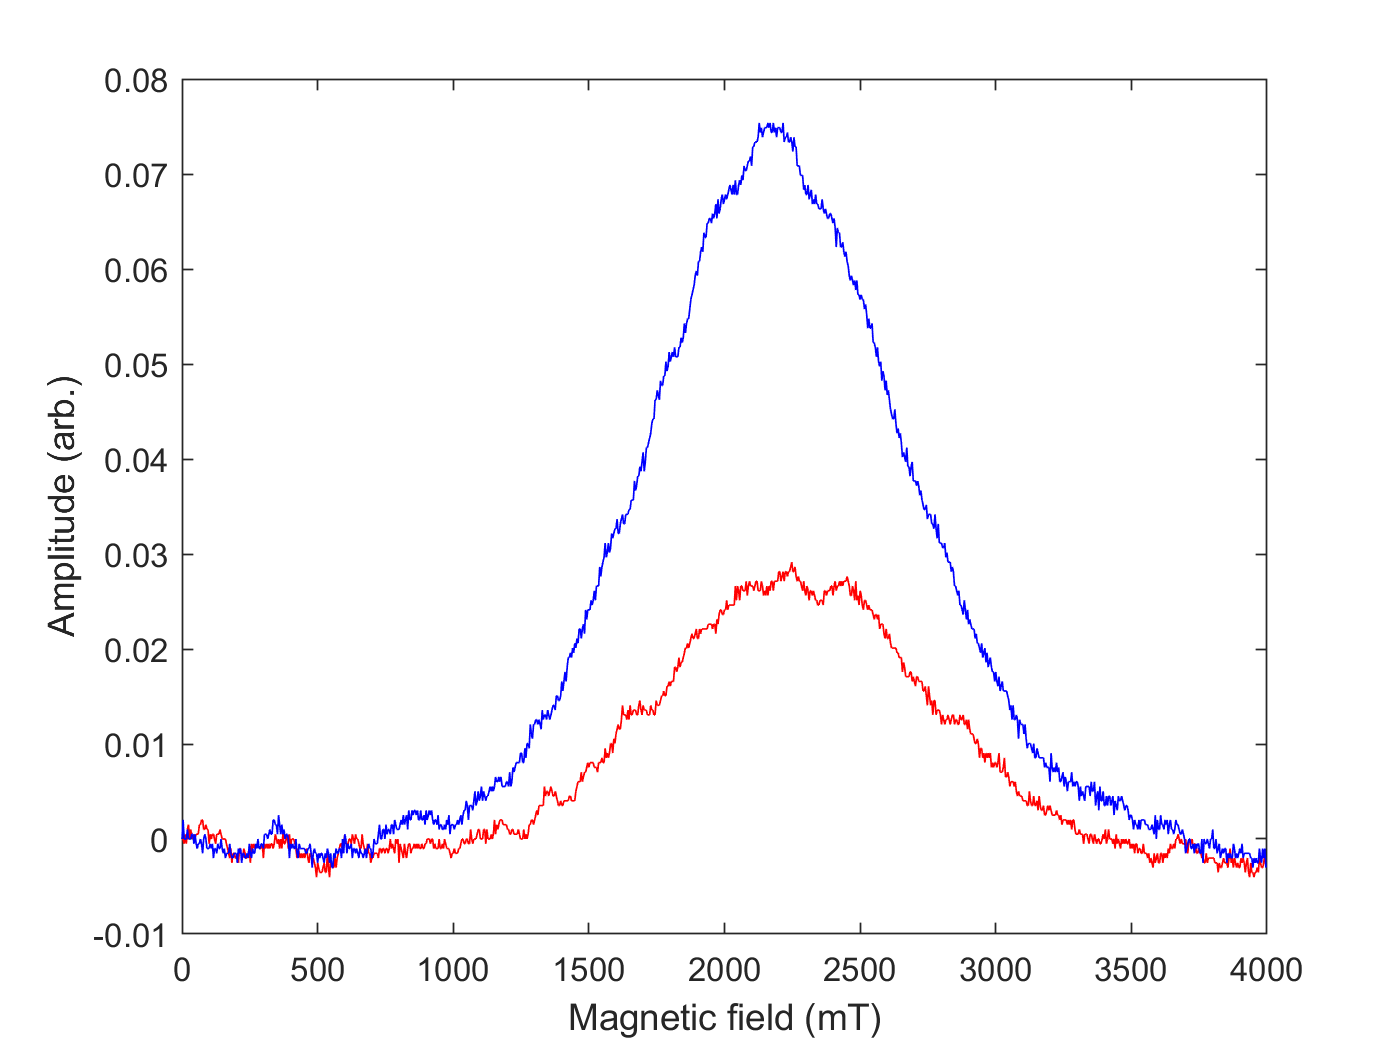
\includegraphics[height=0.5\textwidth,keepaspectratio]{cleanecho}
\caption{\label{fig:cleanecho} $^{171}$Yb$^{3+}$:YSO site II single-shot echo detection. The in-phase (I) and out-of-phase (Q) signals are shown in blue and red, respectively.}
\end{figure}


\begin{figure}[h]
\centering
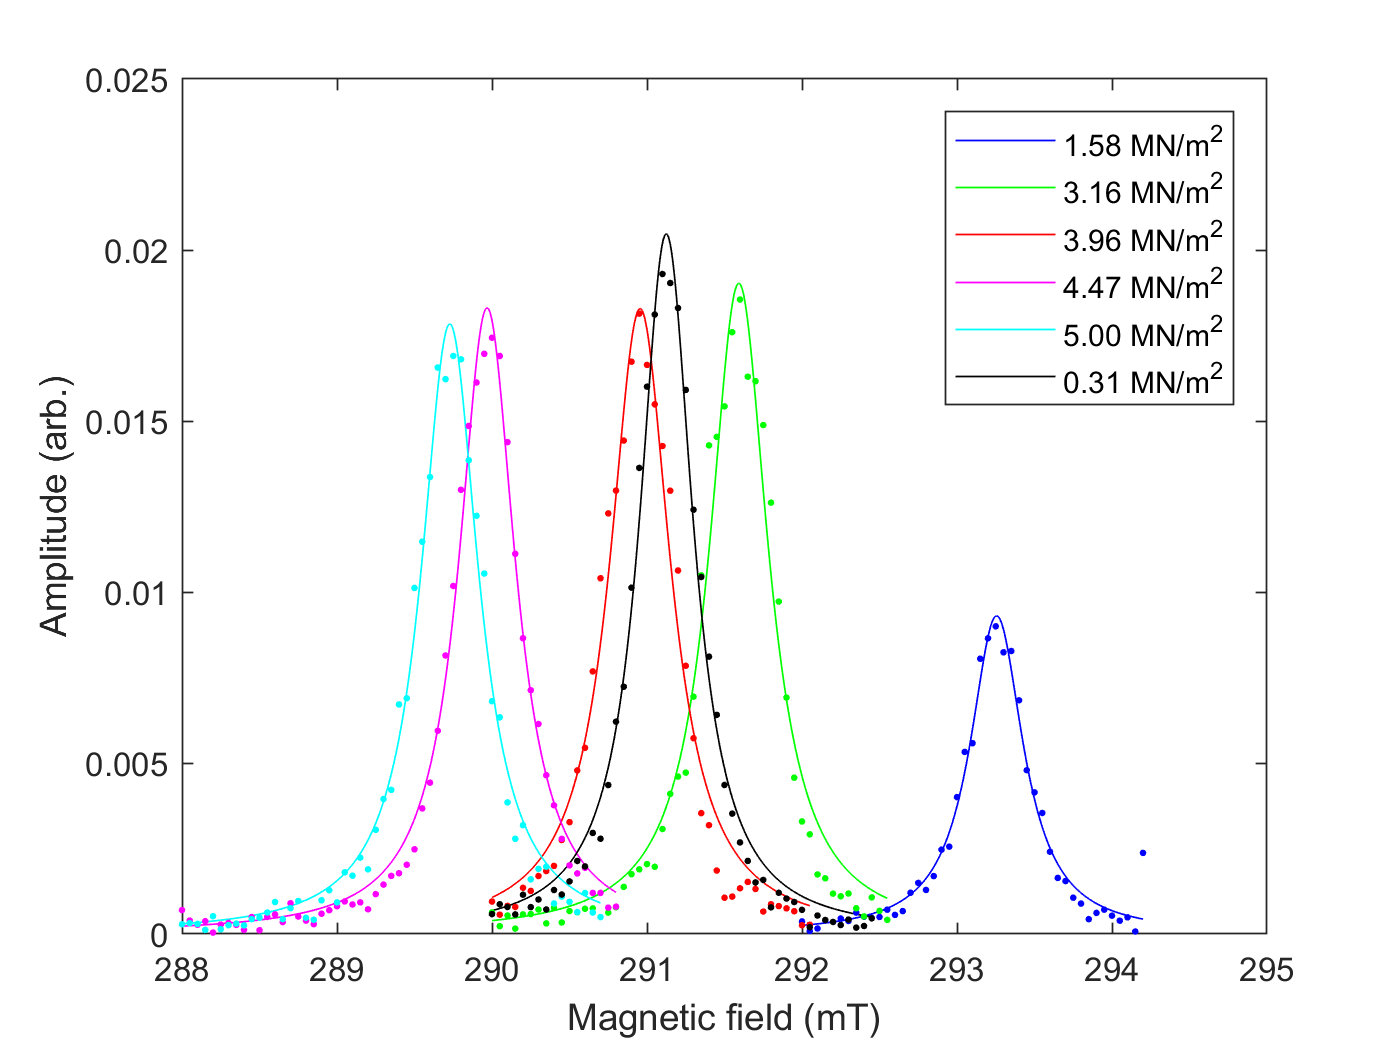
\includegraphics[height=0.5\textwidth,keepaspectratio]{0gfittingpeaks}
\caption{\label{fig:0gfittingpeaks} $^{171}$Yb$^{3+}$:YSO resonance peak for a site II transition as the unaxial stress is increased. The b-axis is perpendicular to $B_{0}$ where $\theta$ = 120.5$\pm 12.4 ^{\circ}$ (or 300.5$\pm 12.4^{\circ}$).}
\end{figure}

\begin{figure}[H]
    \centering
    \begin{subfigure}[b]{0.45\textwidth}
        \centering
        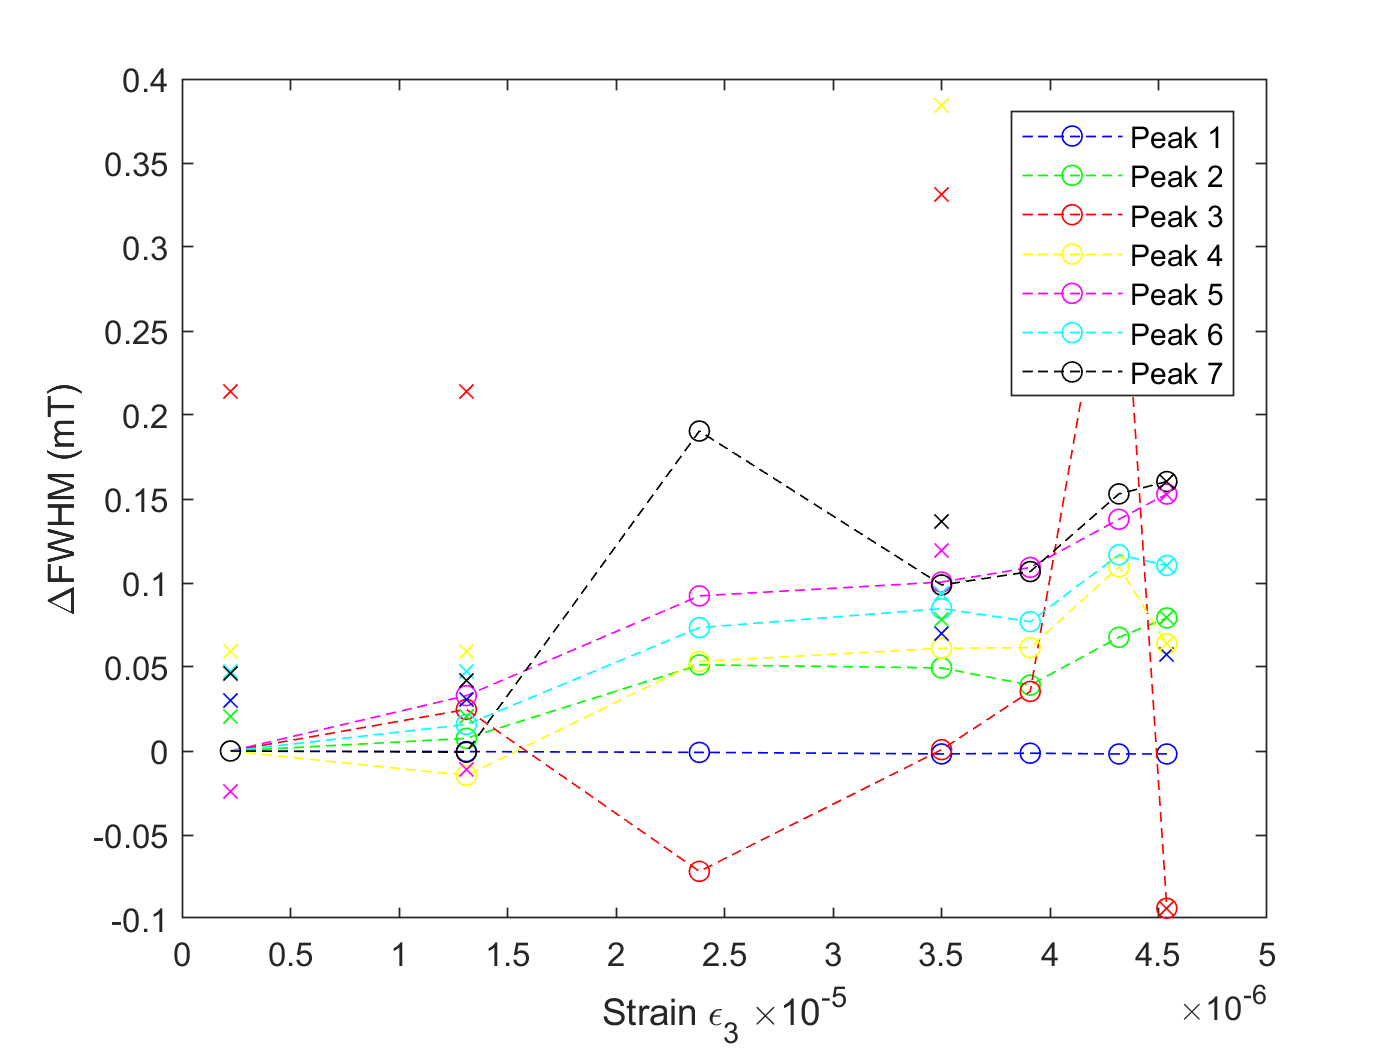
\includegraphics[width=\textwidth]{strainexpthird2}
        \caption{\label{fig:strainexpthird2}}
    \end{subfigure}
%     \hfill
    \begin{subfigure}[b]{0.45\textwidth}
        \centering
        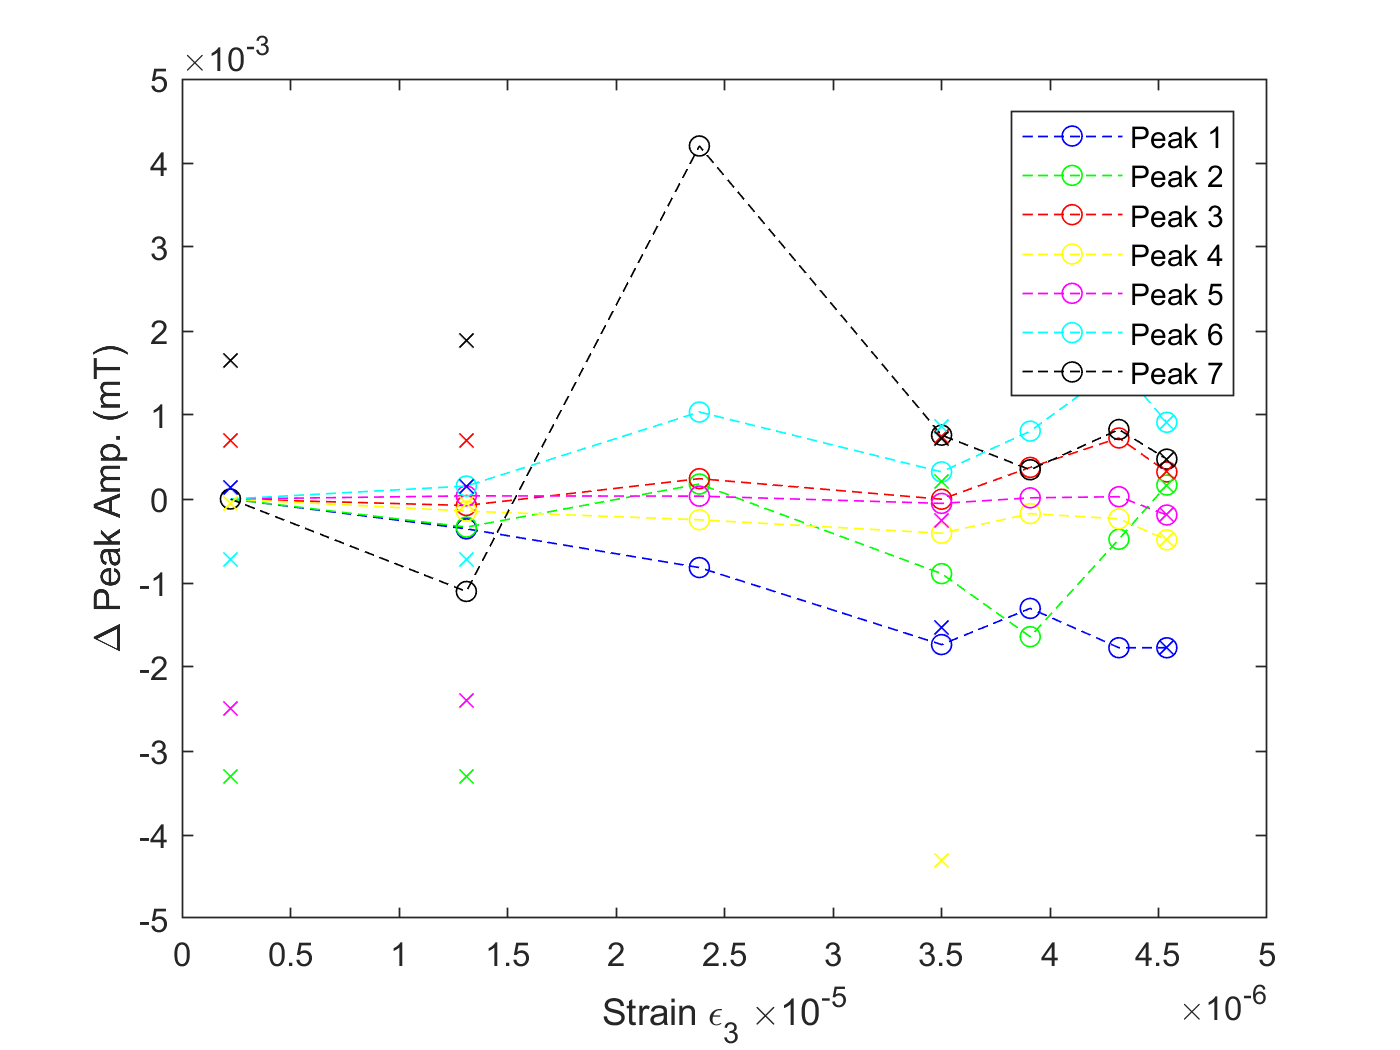
\includegraphics[width=\textwidth]{strainexpthird3}
   \caption{\label{fig:strainexpthird3}}
   \end{subfigure}
   \caption{Yb:YSO site II EPR transitions for $\theta$ = 139.5$\pm 4^{\circ}$ (or 319.5$\pm 4^{\circ}$) from $D1$ in the $D1D2$ plane. (a) Change in the EPR linewidth (full width half maximum FWHM) vs. $\epsilon_{3}$. (b) Change in the resonance signal amplitude vs. $\epsilon_{3}$.}
\end{figure}
